\section{Protocolo In-Band}
\label{sec:ana_inband}

En esta sección, se tomará la decisión de seleccionar el protocolo de control in-band que se utilizará en el proyecto. Después de una cuidadosa evaluación de las opciones disponibles, se ha decidido utilizar el protocolo IoTorii \cite{rojas2021outperforming}, basado en el enfoque de enrutamiento jerárquico, como la solución más adecuada. Esta elección se respalda por el hecho de que el autor del proyecto ha participado activamente en el desarrollo del protocolo IoTorii, lo que garantiza un conocimiento profundo y una experiencia práctica en su implementación.\\
\\
El protocolo IoTorii ofrece una serie de ventajas significativas para el control in-band en entornos de \gls{iot}. Su enfoque jerárquico de etiquetado permite una gestión eficiente y escalable de la red, al tiempo que proporciona una mayor flexibilidad y adaptabilidad a las necesidades específicas del proyecto. Además, IoTorii ha sido probado y validado en diversas situaciones y escenarios, demostrando su eficacia y confiabilidad en la práctica.\\
\\
En este contexto, se ha tomado la decisión de hacer uso de los caminos generados por el protocolo IoTorii, donde cada nodo de la red posee rutas distintas para alcanzar el nodo raíz de la topología. En el caso de este proyecto, el nodo raíz se designará como el controlador (o el nodo que brinda acceso al controlador). Por lo tanto, la innovación radica en la implementación de IoTorii en un entorno de redes definidas por software (SDN).La integración de IoTorii con el entorno SDN permitirá aprovechar las capacidades y ventajas de ambos enfoques. La combinación de la eficiencia y escalabilidad jerárquica de IoTorii con la flexibilidad y el control centralizado de SDN ofrece un enfoque prometedor para el desarrollo y la gestión de redes \gls{iot}. Este enfoque innovador proporcionará una base sólida para llevar a cabo el proyecto y permitirá explorar nuevas posibilidades y mejoras en el ámbito del control in-band para entornos de \gls{iot}.

\subsection{Protocolo IoTorii}

El protocolo IoTorii fue diseñado para trabajar en redes de baja capacidad en entornos \gls{iot}, tratando de solventar carencias de otros protocolos del mismo ámbito como \gls{rpl}, basándose en dos principios: (1) Intercambiar menos mensajes y reducir el tamaño de las tablas de rutas, y (2) Ofrecer resiliencia a través de caminos de \textit{back-up}, con una exploración inicial relativamente rápida. Dichos principios básicos tratan de impactar sobre el consumo y la robustez de las redes de baja capacidad, factores clave en este tipo de redes.


\subsubsection{Operativa del protocolo IoTorii}

El objetivo de IoTorii es dar cada nodo de la red por lo menos una etiqueta jerárquica, en adelante \gls{hlm}, para establecer una jerarquía en la topología. Otra forma de verlo puede ser ver la jerarquía como un árbol que se va ramificando, y está enraizado en el nodo que actúa como \textit{root}. Las \gls{hlm} tratan de proveer de más significado a las MACs convencionales. IoTorii está basado en el protocolo GA3 \cite{rojas2017ga3}, el cual trataba de buscar el mismo etiquetado jerárquico pero en redes cableadas de Data Centers. El principio de estas etiquetas está basado en una revisión del estandar \texttt{ieee802} que se hizo para dar cabida al uso de direcciones MAC mejoradas para el reenvío de paquetes en red.\\
\\
El proceso de la difusión de dichas etiquetas se pueden ver en la figura \ref{fig:iotorii-operation}. El primer paso es establecer en la topología quien va a actuar como nodo \textit{root}, este caso según se puede apreciar es el nodo \texttt{A}. Este nodo será el encargado de iniciar todo el proceso de asignación de etiquetas en la topología. La asignación de etiquetas empezará desde el \textit{root} haciendo uso de un mensaje de tipo \textit{SetHLMAC}, el cual consiste en mandar la \gls{hlm} del remitente más un sufijo que se asociará al vecino. Pero, ¿A qué consideramos vecino? La condición de vecino se da cuando dos nodos se encuentran en rango de cobertura, y se han notificado entre ellos de su presencia mediante un mensaje de tipo \textit{Hello}. Dicho mensaje es una trama vacía donde solo anuncian su dirección MAC real. \\
\\
Un símil en la vida real podría verse como cuando una nueva familia llega al vecindario y va casa por casa presentándose, ``¡Hola somos nuevos aquí {\DejaSans 😃}! Acabamos de llegar al vecindario, nos hemos mudado a la casa de enfrente". Sin embargo, no te sueles presentar con todas las personas del vecindario, solo con los vecinos más cercanos, pporqueno te interesa que todos sepan de ti, solo aquellos con los que vayas a tener relación por cercanía.\\
\\
\begin{figure}[ht!]
    \centering
    \includegraphics[width=\textwidth]{archivos/img/analisis/iotorii-operation.pdf}
    \caption{Operativa del protocolo de IoTorii \cite{rojas2021outperforming}}
    \label{fig:iotorii-operation}
\end{figure}

Por tanto, según se ha explicado, habrá dos tipos de mensajes en este protocolo los mensajes de tipo \textit{Hello} y de tipo, \textit{SetHLMAC}. Este último, recordemos que asigna una nueva \gls{hlm}, la cual se compone de la \gls{hlm} del remitente más un sufijo único que se asocia al vecino en cuestión. Por ejemplo en la figura \ref{fig:iotorii-operation}, el nodo \texttt{A} asigna a sus vecinos los sufijos $\texttt{1,2,3,4,5}$, por lo que las  \gls{hlm} que mandará respectivamente serán las siguientes, $\texttt{[1.1],[1.2],[1.3],[1.4],[1.5]}$. Dichos sufijos únicos por vecino se van asignando según se reciben mensajes de tipo \textit{Hello}, por lo que, se va construyendo una asociación de MAC real con sufijo único.\\
\\
Los mensajes de tipo \textit{Hello} se tienen que transmitir de forma periódica para que todo el mundo tenga actualizado su lista de vecinos, ya que en este caso no se tiene una red cableada donde las relaciones entre los nodos son constantes, sino, nodos en un escenario inalámbrico, por lo que movilidad es inherente. Por ello, de forma periódica se tiene que reafirmar que sigues siendo vecino de tus nodos adyacentes. Volviendo al símil de la vida real, podría verse como que el vecindario en vez de ser casas al uso, son caravanas, las cuales tienen la capacidad de aparcar donde quieran del vecindario, por lo que de vez en cuando tienes que presentarte de nuevo porque puede que los vecinos que tengas no sean los mismos.\\
\\
Cuando un nodo recibe un mensaje de tipo \textit{SetHLMAC}, lo almacenan en su  tabla de posibles rutas al nodo raíz, y lo reenvían a todos sus posibles vecinos poniendo sus respectivos sufijos únicos. Este proceso se lleva a cabo de forma iterativa hasta que se han difundido todas las posibles \gls{hlm} o hasta que se haya llegado al número máximo de \gls{hlm} por nodos (parámetro configurable del protocolo). Por ejemplo, si nos fijamos de nuevo en la figura \ref{fig:iotorii-operation}, podemos ver como siguiendo con este proceso el nodo \texttt{B} recibe del nodo root la \gls{hlm} $\texttt{[1.5]}$, por lo que, una vez almacenada la etiqueta la difundirá a todos sus posibles vecinos. El nodo \texttt{B} generará las etiquetas $\texttt{[1.5.8],[1.5.1],[1.5.3]}$, y las mandará a sus nodos vecinos. La etiqueta $\texttt{[1.5.8]}$ le llegará al nodo \texttt{C} desde el nodo \texttt{B}, pero también le llegará la etiqueta $\texttt{[1.3.2.8]}$ a través del nodo \texttt{B} (como se puede ver el sufijo es el mismo en ambos casos), las guardará y las dinfundirá a todos sus vecinos. Para prevenir bucles solo hay que inspeccionar si la \gls{hlm} que te llega es hija de algunas que tienes guardadas en tu tabla de rutas. Por ejemplo, el nodo \texttt{B} descartará todas \gls{hlm} que le lleguen siguiendo el formato $\texttt{[1.5.X.Y]}$ o $\texttt{[1.3.2.X.Y]}$. Todo este proceso de difusión de etiquetas \gls{hlm} se encuentra descrito en el bloque de algoritmo \ref{iotorii-alg}.\\
\\
Una vez convergida la difusión de etiquetas \gls{hlm}, se tendrá construido un árbol enraizado en el nodo establecido como \textit{root}, y cada hoja del árbol tendrá una o más rutas para alcanzar al \textit{root}.

\newpage

\begin{algorithm}[ht!]
    \SetAlgoLined
    %\KwResult{Write here the result }
    % initialization\;
    send \textit{Hello}\;
    \While{frame received}{
        %instructions\;
        \uIf{Hello}{
            \eIf{MAC not in Hello table}{
                assign unique \textit{suffix}\;
                save tuple \{\textit{MAC,suffix}\}\;
                \If{root node}{
                    create \textit{SetHLMAC} with HLMAC=1\;
                    \For{each tuple in Hello table}{
                        add tuple to \textit{SetHLMAC}\;
                    }
                    broadcast \textit{SetHLMAC}\;
                }
            }{
                discard\;
            }
        }
        \uElseIf{SetHLMAC}{
            \eIf{HLMAC (or prefix) not in HLMAC table}{
                save HLMAC in \textit{HLMAC table}\;
                create \textit{SetHLMAC} with received HLMAC\;
                \For{each tuple in Hello table}{
                    add tuple to \textit{SetHLMAC}\;
                }
                broadcast \textit{SetHLMAC}\;
            }{
                discard\;
            }
        }
        \Else{
            discard\;
        }
    }
    \caption{Assignment of HLMACs in IoTorii}
    \label{iotorii-alg}
\end{algorithm}


\subsubsection{Configuración del protocolo IoTorii}

La difusión de las \gls{hlm}s puede ser configurada para ajustarse mejor sobre la red que se vaya a trabajar. Se han dejado tres parámetros de diseño.

\begin{itemize}
    \item Longitud de \gls{hlm}, establece como de larga podrá ser una etiqueta \gls{hlm}. Este parámetro nos indica a cuantos saltos estaremos desde una hoja del árbol, al nodo raíz.
    \item Número de bits para sufijos únicos, es decir, que amplitud de \gls{hlm} vamos a tener. Esto definirá cuantos vecinos recibirán etiquetas desde un nodo dado. Por ejemplo, si tenemos 2 bits, podremos dar cabida hasta 4 vecinos.
    \item Número de \gls{hlm}, indica el número de rutas máximo que cada nodo guardará en su tabla de rutas al \textit{root}.
\end{itemize}

Todos los parámetros anteriormente mencionados afectarán también sobre el tamaño de la trama generada de tipo \textit{SetHLMAC}, la cual se puede apreciar en la figura \ref{fig:frameformat-setHLMAC} Otro parámetro configurable es la periodicidad de los mensajes de tipo \textit{Hello}, los cuales son fundamentales para gestionar la movilidad de los nodos en la red.

\begin{figure}[ht!]
    \centering
    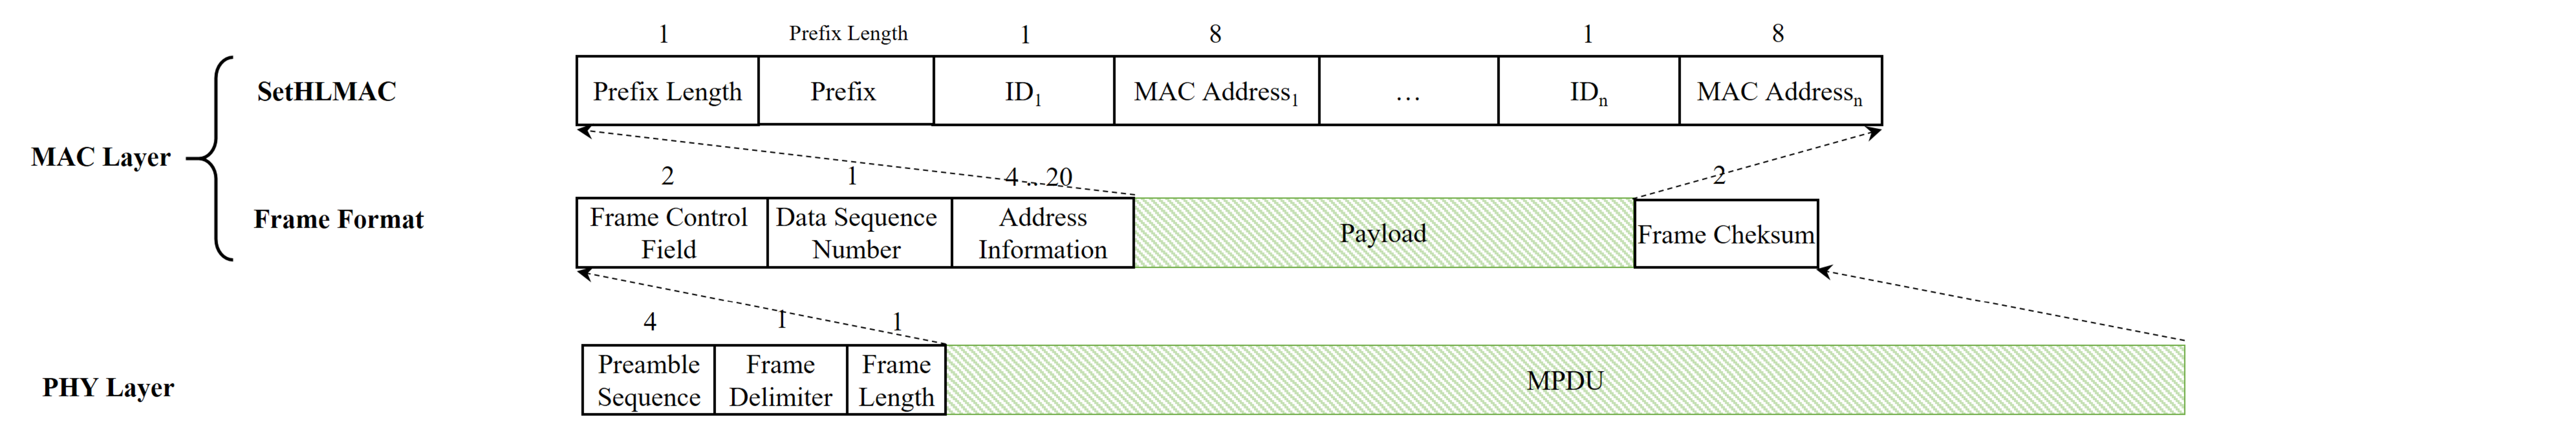
\includegraphics[width=\textwidth]{archivos/img/analisis/Comparation_frame_iotorii.eps}
    \caption{Mensajes de control en IoTorii \cite{rojas2021outperforming}}
    \label{fig:frameformat-setHLMAC}
\end{figure}